\chapter[Proposal]{Proposal}

This proposal focuses on detailing the necessary steps to the creation and publication of a crowdfunding speech corpus in Brazilian Portuguese. To this end, a virtual voice recording application will be developed (section \ref{sec:proposal-app}), focusing on adding gamification elements to enhance user engagement. Additionally, this application will also extract some relevant characteristics found in the systematic literature review in chapter \ref{chap:slr}. Once the construction is finished, the application will be released, allowing general public submission (in section \ref{sec:proposal-public-submission}). After the submission period, the collected data will be analyzed and compiled to a speech corpus (\ref{sec:proposal-data-analysis}), which will be publicized to an open-source repository in section \ref{sec:proposal-data-publication}.

\section{Application}
\label{sec:proposal-app}

This section details the conception, documentation, and development process of the voice recording application, coined "Fale Alguma Coisa". Below, it will at times be referenced as "app", short for application.

\begin{figure}[ht]
    \centering
    \caption{Fale Alguma Coisa app Logo}
    
\includegraphics[width=\linewidth/2]{images/app/logo.jpg}
    \caption*{Source: Author}
    \label{fig:falealgumacoisa-logo}
\end{figure}

\subsection{Concept}

The Fale Alguma Coisa app should provide an easy gateway for you to contribute your voice while having fun and learning various science facts and curiosities.

\subsection{Target Audience}

Directed towards anyone interested in learning and contributing to science.

\subsection{User Stories}

The development of most software starts with its documentation. This work chose a user story approach to project documentation and lists them below, categorized by epic.

\subsubsection{Usability}

\begin{itemize}
    \item I, as a citizen, would like to contribute my voice using my mobile devices and desktop computer.
\end{itemize}

\subsubsection{Homepage}

The homepage epic represents the user stories affecting the homepage, such as the splash screen, call to action button, terms of service, etc.

\begin{itemize}
    \item I, as an unregistered citizen, would like to view an animated introductory screen in the application, so that I feel more inside a native app.
    \item I, as an unregistered citizen, would like to know more about Fale Alguma Coisa from a explanatory text in the homepage, so that I understand more about the project.
    \item I, as a registered citizen, would like to easily go from the homepage to the sign-in page, so that I can login to my account.
    \item I, as an unregistered citizen, would like to click a call to action button to go from the homepage to the recording page from the homepage, so that I can contribute my voice.
    \item I, as an unregistered citizen, would like to read the terms of service and privacy policy of Fale Alguma Coisa, so that I understand better what the service has to offer and what kind of data will be recorded.
\end{itemize}

\subsubsection{Recording}

The recording epic represents the most important feature in the application, as the citizen will use it to record his voice. It also provides supporting features, such as skipping phrases and resuming the recording session.

\begin{itemize}
    \item I, as an unregistered citizen, would like to view and accept the terms of service before recording, so that I understand how my data is being used.
    \item I, as an unregistered citizen, would like to properly configure my microphone before recording, so that I can record without interruption.
    \item I, as a citizen, would like to read science phrases with definitions and curiosities, so that I learn about subjects as I am contributing.
    \item I, as a citizen, would like to read phrases grouped by theme, so that I can learn more from each subject as I am contributing.
    \item I, as a citizen, would like to read a tutorial explaining how to record, so that I learn how to properly record phrases.
    \item I, as a citizen, would like to see animations on each step of the recording (enter the page, start the recording, stop the recording), so that I feel more engaged with the application.
    \item I, as a citizen, would like to skip a phrase when I (1) do not know how to pronounce, or (2) find a foreign word, or (3) another specified reason, so that I only speak the correct phrases.
    \item I, as a unregistered citizen, would like to stop this recording session by returning home when clicking the logo and confirming the exit, so that I can resume it afterwards.
    \item I, as a registered citizen, would like to return to the dashboard after clicking the logo and confirming the exit, so that I can resume it afterwards.
\end{itemize}

\subsubsection{Dashboard}

The dashboard epic lists all user stories related to the dashboard page, where the user will be able to choose themes to record, open the menu, check his level, etc.

\begin{itemize}
    \item I, as an unregistered citizen, would like to easily register my data through a button click, so that I can enjoy all features of the logged area.
    \item I, as a registered citizen, would like to see my actions in a dashboard after logging in, so that I can better contribute to the project.
    \item I, as a registered citizen, would like to see a list of recommended themes to speak, so that I can choose one from the list.
    \item I, as a registered citizen, would like to view my progress level, so that I know how far have I progressed in my contributions.
    \item I, as a registered citizen, would like to open the menu, so that I know which are my possible actions in the app.
    \item I, as a registered citizen, would like to check notifications, so that I understand what happened while I was gone.
\end{itemize}

\subsubsection{Gamification}

\begin{itemize}
    \item I, as a registered citizen, would like to get 100 points when I record my first phrase, so that I can engage better in the application.
    \item I, as a registered citizen, would like to get 400 points when I record my first theme, so that I can engage better in the application.
    \item I, as a registered citizen, would like to get 300 points when I record subsequent themes, so that I can engage better in the application.
    \item I, as a registered citizen, would like to get 500 points when I register my data, so that I can better engage with the application.
    \item I, as a registered citizen, would like to measure my points through a level, so that I can more easily compare myself with other users.
\end{itemize}

\subsubsection{Social}

\begin{itemize}
    \item I, as a registered citizen, would like to know who are the top contributors in the space and where am I in the list, so that I can compete against them.
    \item I, as a registered citizen, would like to know where my friends are in a more customized leaderboard, so that I can compete against them.
    \item I, as a registered citizen, would like to add a friend, so that I can check them in the friends leaderboard afterwards.
    \item I, as a registered citizen, would like to check notifications, so that I can know what happened when I was away.
    \item I, as a registered citizen, would like to know when someone added me through notifications, so that I can add them back later.
    \item I, as a registered citizen, would like to refer friends to the application, so that I can play with them.
\end{itemize}

\subsubsection{Login and Registration}

\begin{itemize}
    \item I, as an unregistered citizen, would like to login (using social login - Facebook / Google) on the app, so that I can login later and save my progress.
    \item I, as a unregistered citizen, would like to register my anonymous data on my first login, so that I can provide better metadata to my recordings afterwards.
    \item I, as a registered citizen, would like to update my account data, so that I can provide accurate metadata to the recordings.
    \item I, as a registered citizen, would like to remove my account data (and my recordings, if necessary), so that I can remove my metadata from this application.
\end{itemize}

\subsection{Design}

To ensure the development of the application is effective, an iterative design approach was taken. First, ideas for the app shaped a conceptual user journey. Second, this journey allowed the creation of layouts, which then passed through a validation process. Then, if aligned with the application concept, the layouts were developed. Otherwise, another design implementation occurred, undergoing further validation.

\subsubsection{Color Scheme}

In color theory, colors are used to communicate meaning, but also affect mood, and perception \cite{agoston2013color}. The design color scheme defines a color palette to choose from when designing new elements. Applying the concept, a more colorful color scheme was chosen to lighten the mood of the application, as shown in figure \ref{fig:falealgumacoisa-color-scheme}.

\begin{figure}[ht]
    \centering
    \caption{Fale Alguma Coisa color scheme}
    
\includegraphics[width=\linewidth/2]{images/app/colors.png}
    \caption*{Source: Author}
    \label{fig:falealgumacoisa-color-scheme}
\end{figure}

\subsubsection{Web app}

To allow easier access to the voice recording app, a web-based application will be developed. This factor positively influences the capacity of the app to update over time, when compared to an application developed in a native environment. It also enables users over mobile and desktop to access the same application, and although the layout may have to be redesigned, most logic is reused.

\subsubsection{Mobile First}

The design will use a mobile first approach, to ensure the user flow will be optimized when he is using a mobile device. The desktop flow will be designed and developed afterwards.

\subsubsection{Splash Screen}

As the user first enter the application, a splash screen will be shown to welcome him (mobile version in figure \ref{fig:falealgumacoisa-splash-page-design}). It contains the logo and an animation to draw the user's attention. After the animation, the home will be shown.

\begin{figure}[ht]
    \centering
    \caption{Fale Alguma Coisa Splash Page design}
    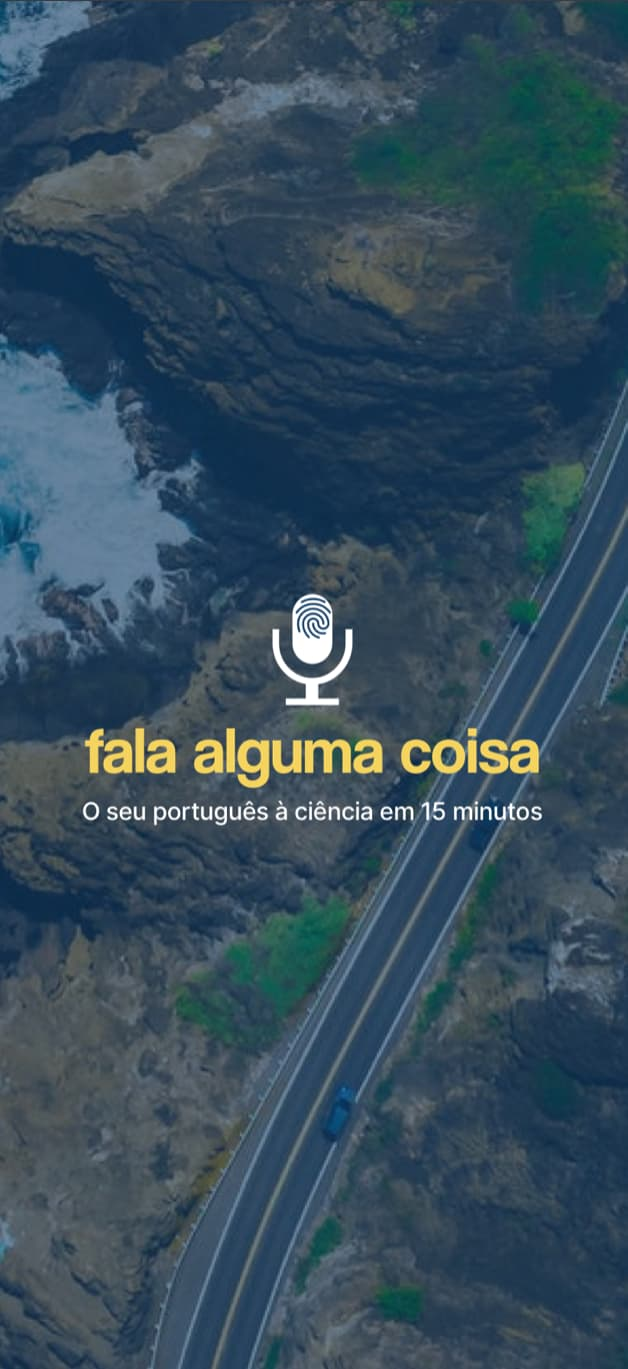
\includegraphics[width=\linewidth/2]{images/app/m-splash.jpg}
    \caption*{Source: Author}
    \label{fig:falealgumacoisa-splash-page-design}
\end{figure}

\subsubsection{Homepage}

After the splash animation, the homepage is shown. The mobile version can be seen below in figure \ref{fig:falealgumacoisa-home-page-design}. In this page, the call to action to start the recording is highlighted by the button at the center of the page, with text describing the project right below it. The login page is accessible through the link in the right upper corner. These few elements are placed to encourage the user to click on the recording, if he is a new user.

\begin{figure}[ht]
    \centering
    \caption{Fale Alguma Coisa Home Page design}
    \frame{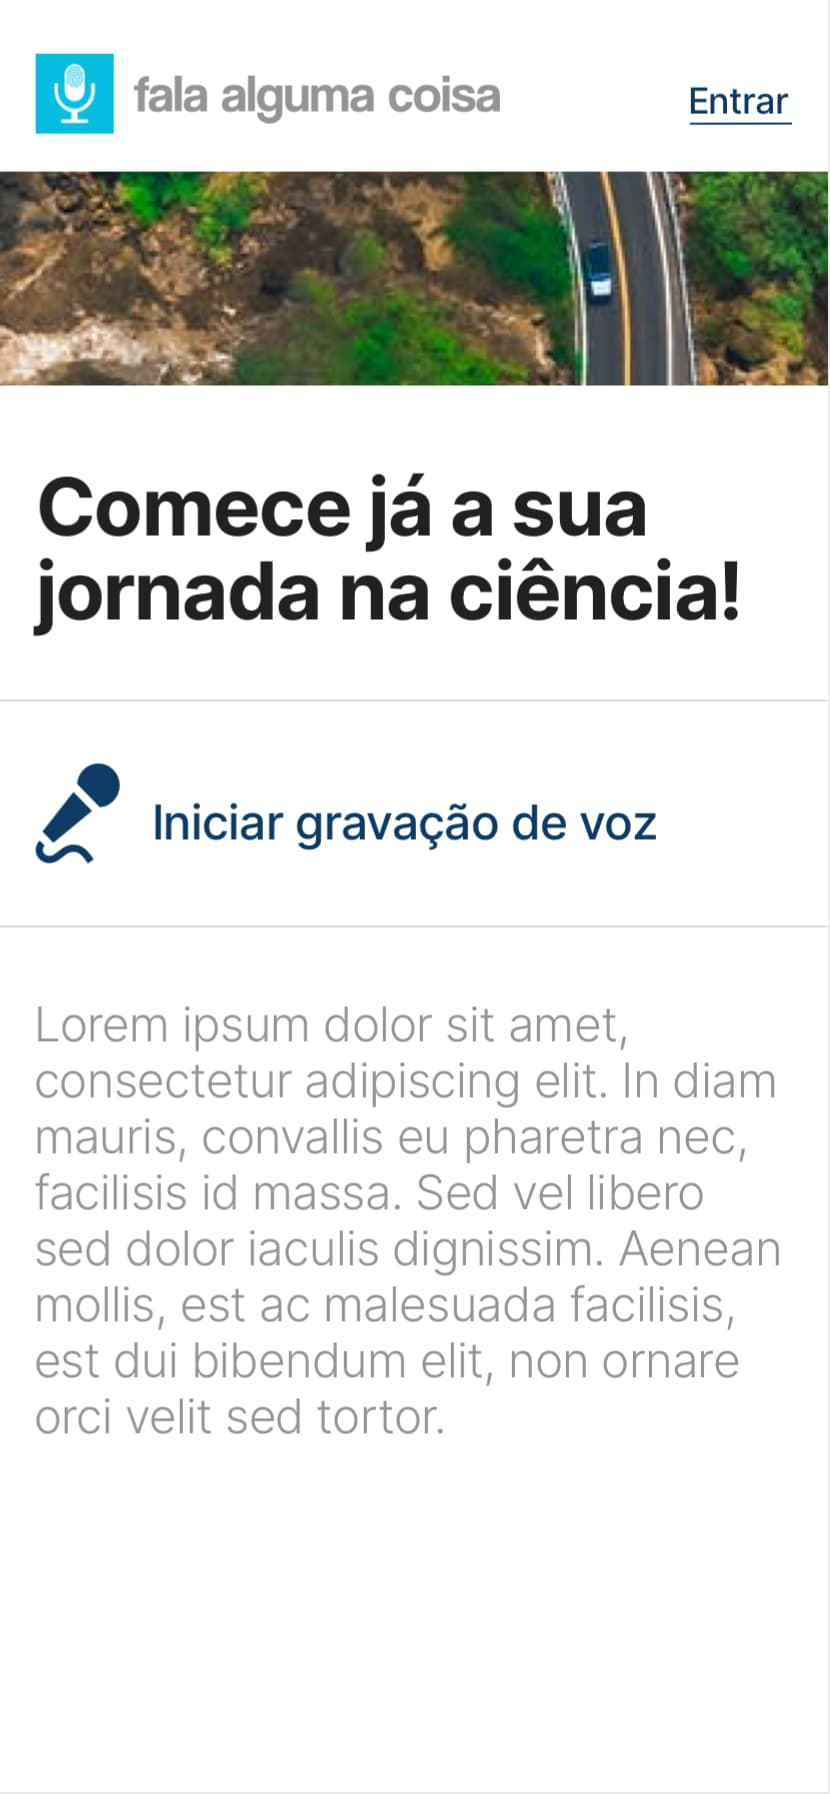
\includegraphics[width=\linewidth/2]{images/app/m-home.jpg}}
    \caption*{Source: Author}
    \label{fig:falealgumacoisa-home-page-design}
\end{figure}

\subsubsection{Recording}

This page represents the core functionality of the website, allowing the user to record phrases with his voice. The recording is done through groups of phrases, called a theme, and is illustrated by the image \ref{fig:falealgumacoisa-recording-page-design} at the bottom. The main elements of the page are (1) the phrase highlighted in a rectangular box at the center of the page, and (2) the red recording button at the bottom.

\begin{figure}[ht]
    \centering
    \caption{Fale Alguma Coisa Recording Page design}
    \frame{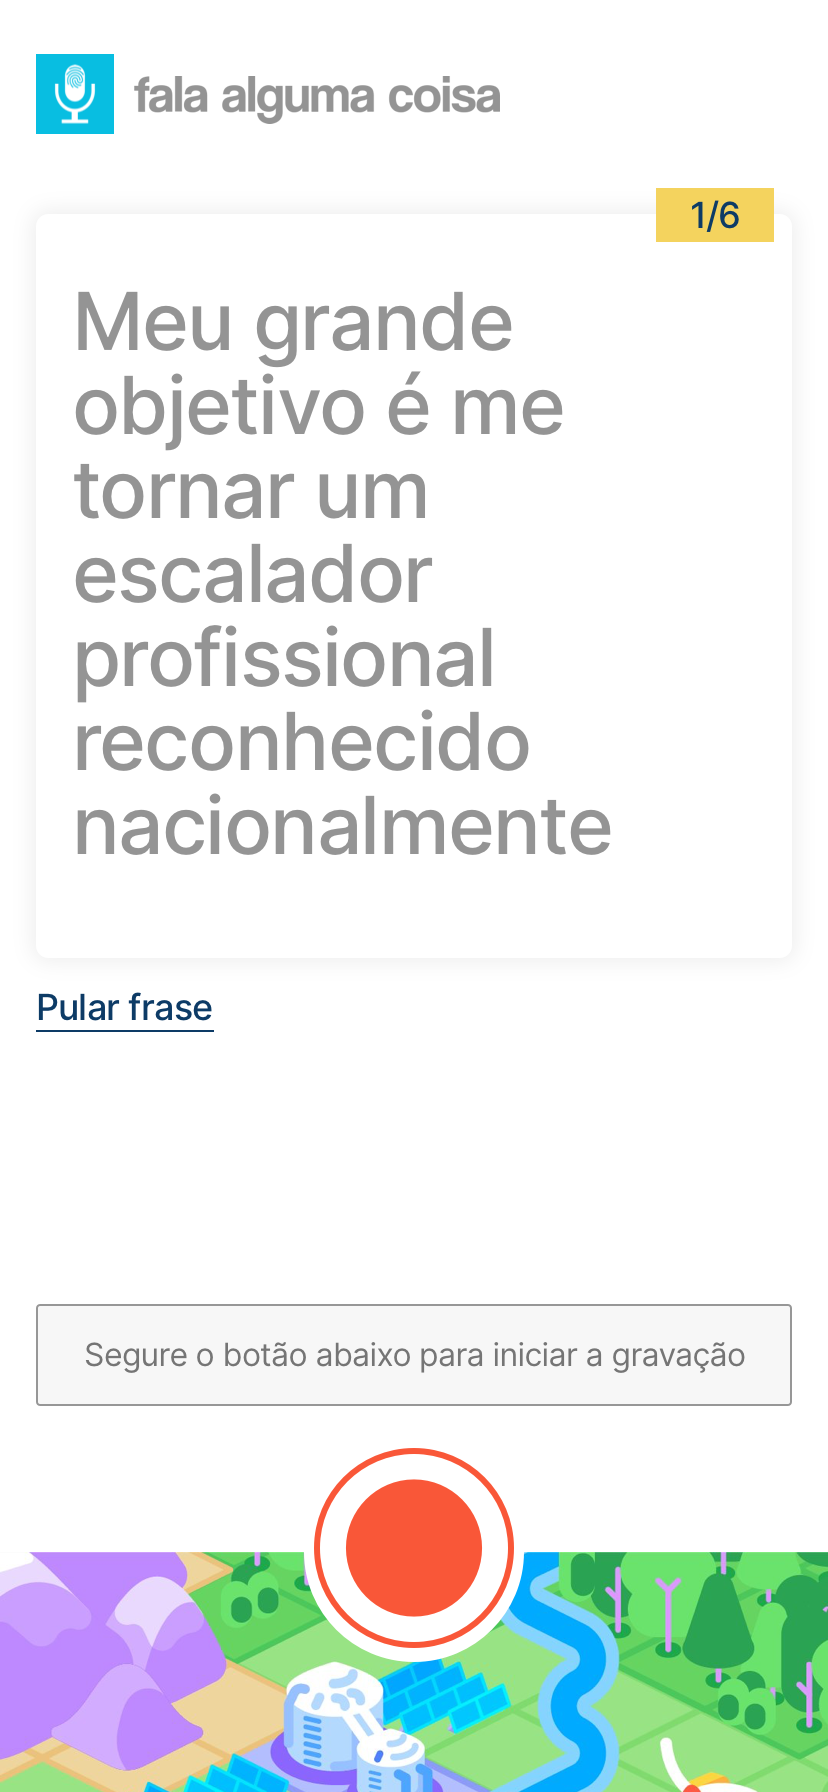
\includegraphics[width=\linewidth/2]{images/app/recording/Journey_1.0.png}}
    \caption*{Source: Author}
    \label{fig:falealgumacoisa-recording-page-design}
\end{figure}

\subsubsection{Dashboard}

When an unauthenticated user finishes recording its first theme, or when a user logs in, they are able to select from a list of themes to record. In this dashboard seen in figure \ref{fig:falealgumacoisa-dashboard-page-design}, they are also shown the number of points accumulated by the usage of the app, as well as able to open a menu and notification page.

\begin{figure}[ht]
    \centering
    \caption{Fale Alguma Coisa Dashboard Page design}
    \frame{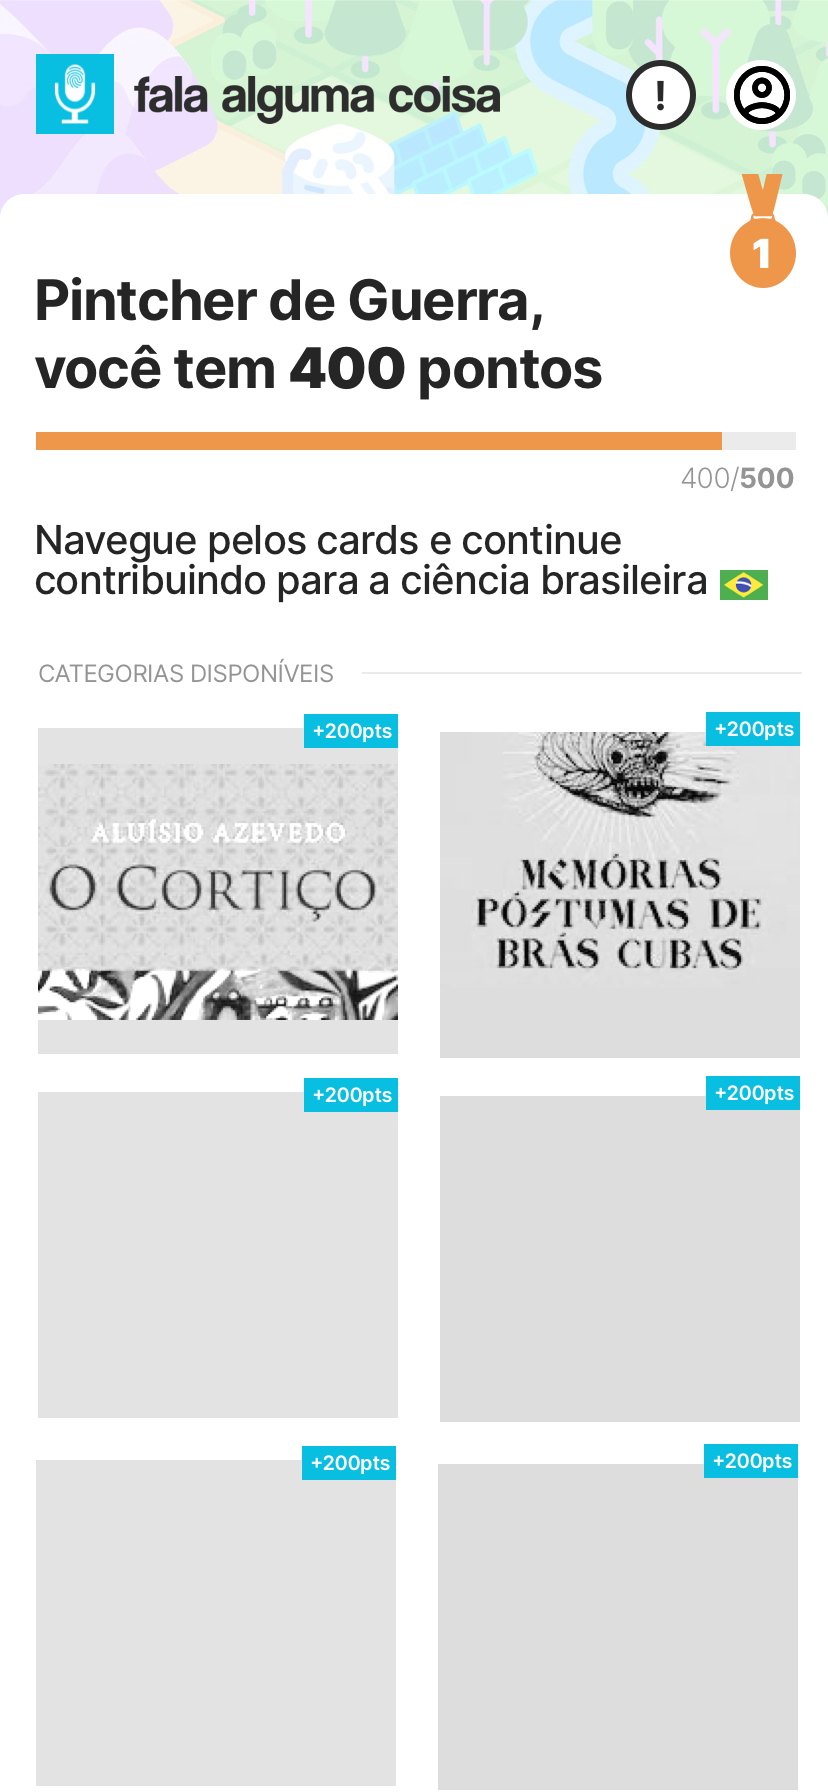
\includegraphics[width=\linewidth/2]{images/app/dashboard/Dashboard.png}}
    \caption*{Source: Author}
    \label{fig:falealgumacoisa-dashboard-page-design}
\end{figure}

\subsubsection{Leaderboard}

The leaderboard has two views: a list of the top ranking users (figure \ref{fig:falealgumacoisa-leaderboard-page-design-general}) and a list of friend rankings (figure \ref{fig:falealgumacoisa-leaderboard-page-design-friend}). They provide a way for users to compare their contributions, thus promoting competition. A social part is also included throughout the option to add friends.

\begin{figure}[ht]
    \centering
    \caption{Fale Alguma Coisa Leaderboard Page designs}
    \begin{subfigure}{.5\textwidth}
      \centering
      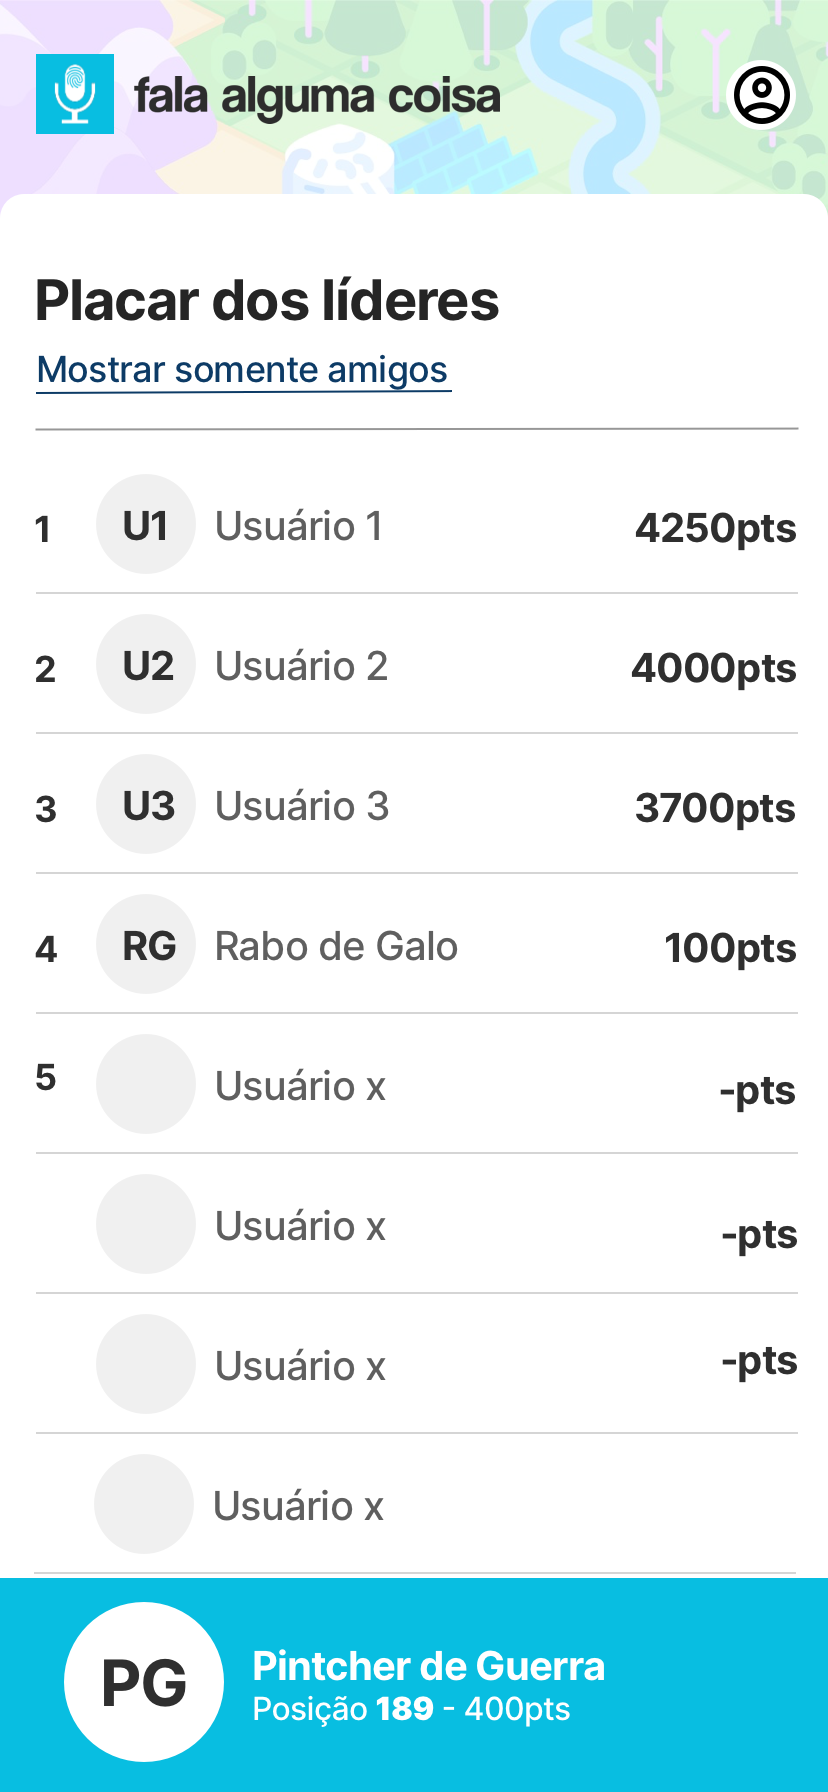
\includegraphics[width=.9\linewidth]{images/app/leaderboard/GeneralRanking.png}
      \caption{General Leaderboard}
      \label{fig:falealgumacoisa-leaderboard-page-design-general}
    \end{subfigure}%
    \begin{subfigure}{.5\textwidth}
      \centering
      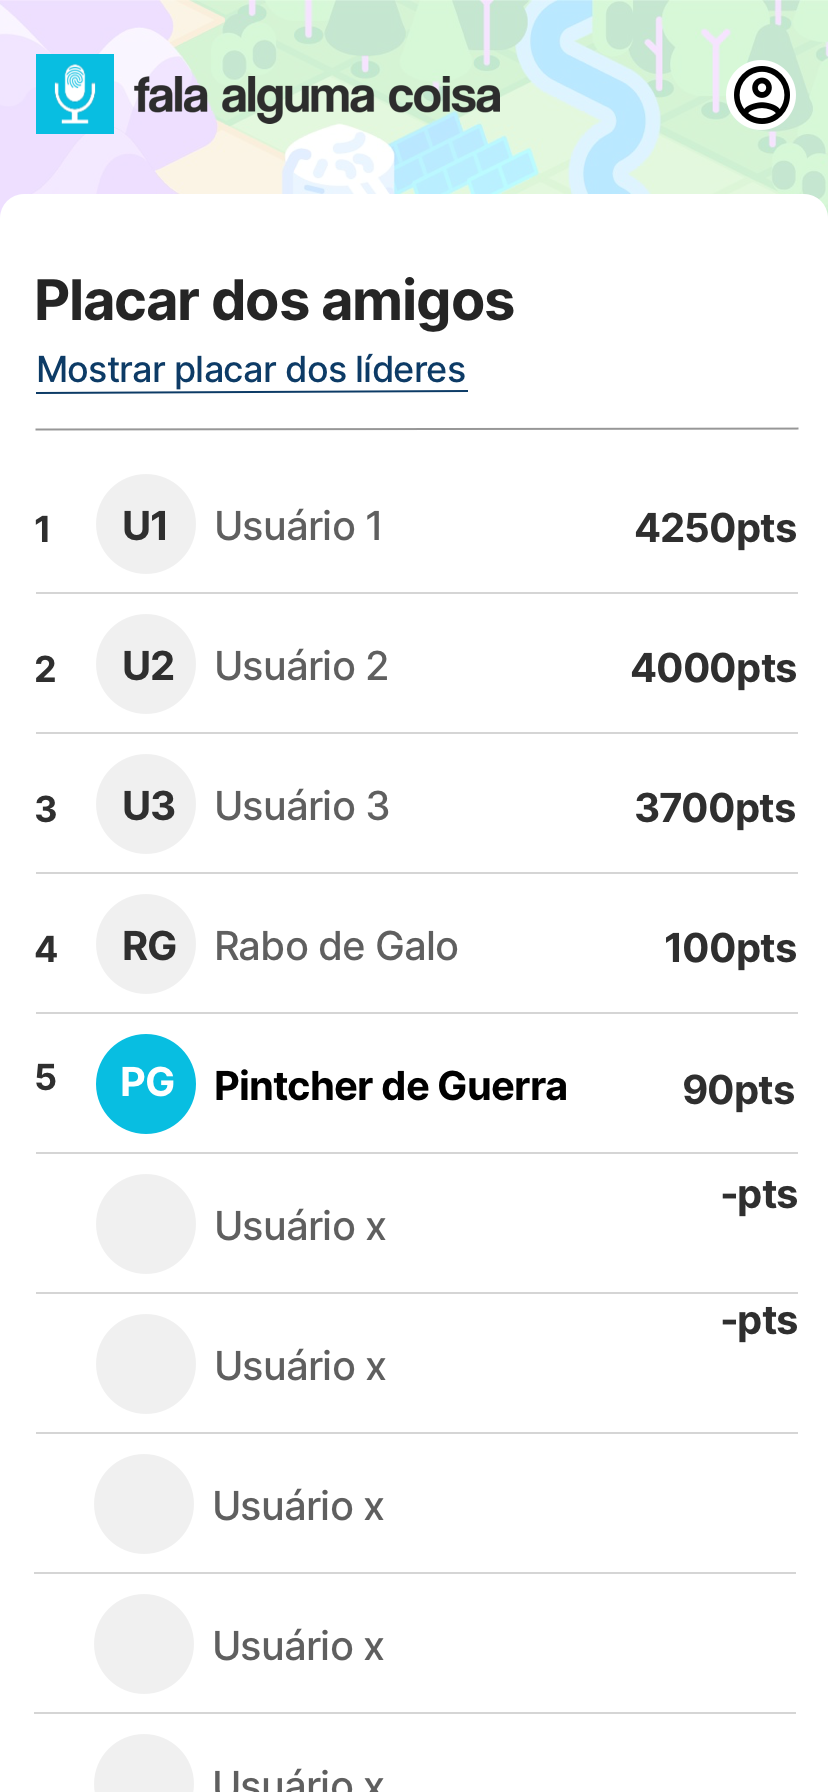
\includegraphics[width=.9\linewidth]{images/app/leaderboard/FriendsRanking.png}
      \caption{Friends Leaderboard}
      \label{fig:falealgumacoisa-leaderboard-page-design-friend}
    \end{subfigure}
    \caption*{Source: Author}
    \label{fig:falealgumacoisa-leaderboard-page-design}
\end{figure}

\subsubsection{Login and Registration}

The login and registration pages include essential features to the application: the ability to identify the user and maintain a history of recordings.

\begin{figure}[ht]
    \centering
    \caption{Fale Alguma Coisa Login and Registration Page designs}
    \begin{subfigure}{.5\textwidth}
      \centering
      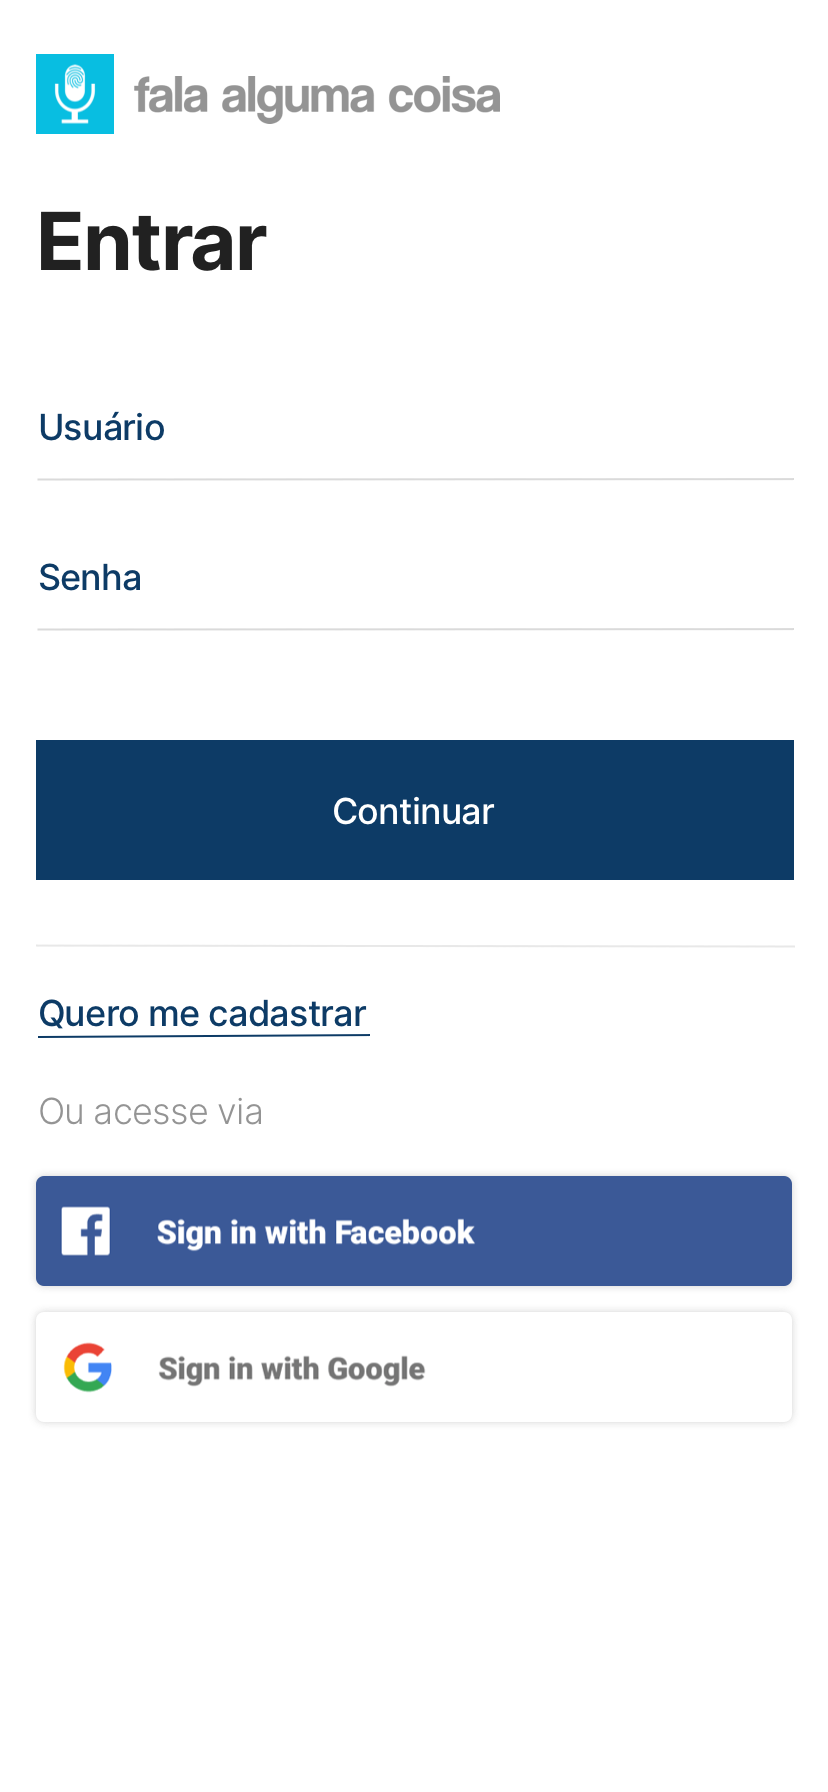
\includegraphics[width=.9\linewidth]{images/app/login/Login1.png}
      \caption{Login Page}
      \label{fig:falealgumacoisa-login-page-design}
    \end{subfigure}%
    \begin{subfigure}{.5\textwidth}
      \centering
      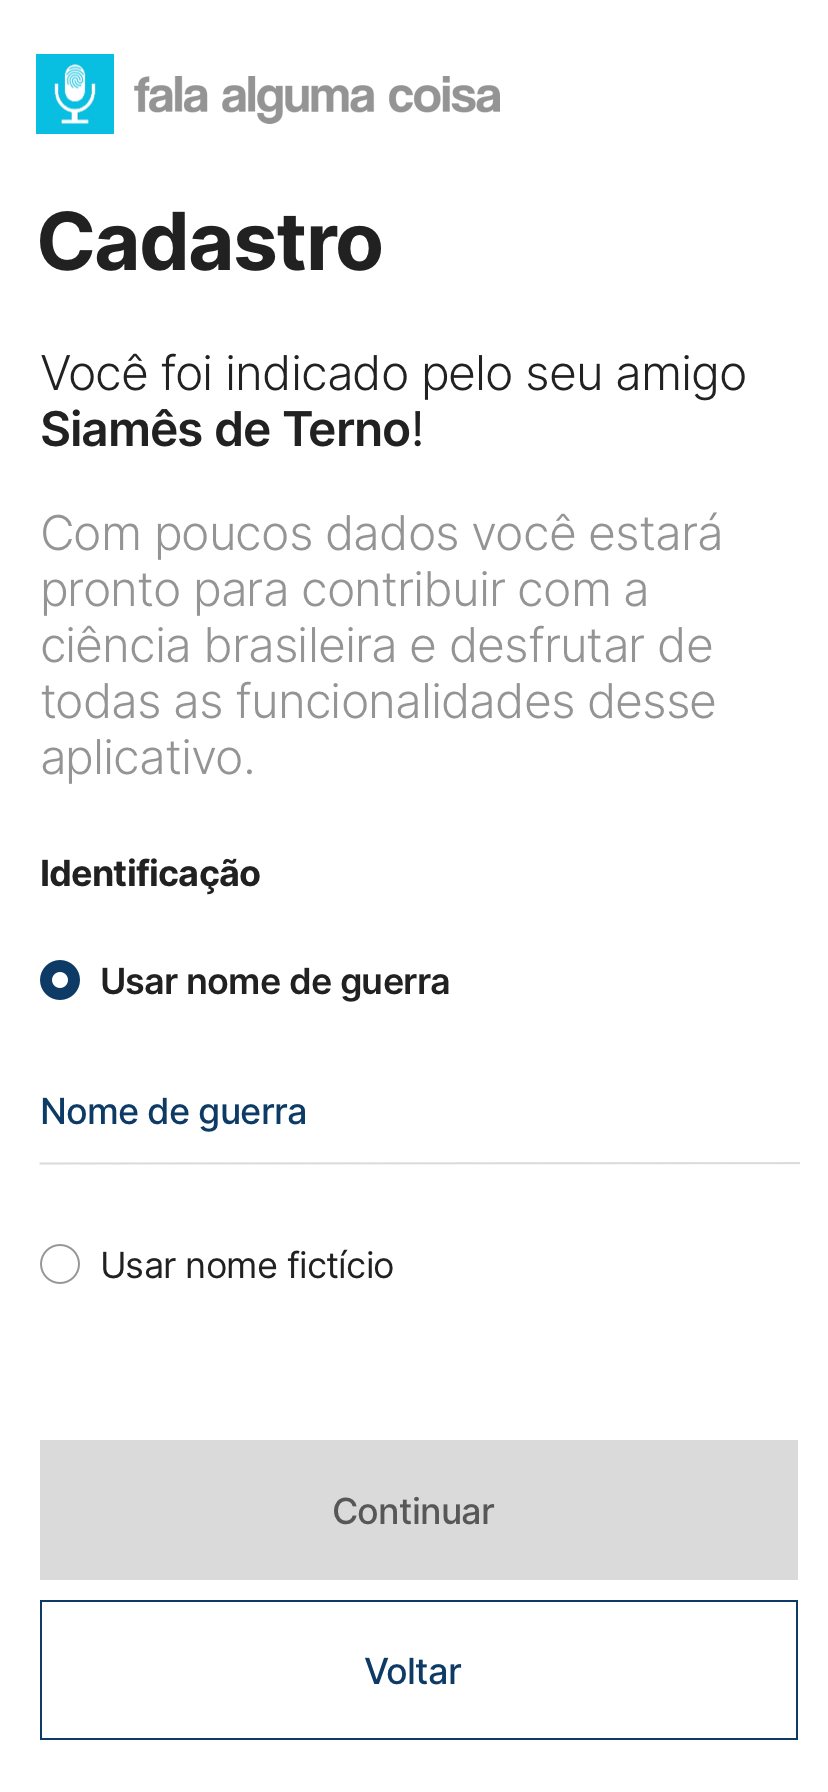
\includegraphics[width=.9\linewidth]{images/app/register/Register1.0.png}
      \caption{Registration Page}
      \label{fig:falealgumacoisa-registration-page-design}
    \end{subfigure}
    \caption*{Source: Author}
    \label{fig:falealgumacoisa-login-page-design}
\end{figure}

\subsubsection{Delete User}

If necessary, the user should be able to delete its user data, while still contributing his voice to the speech corpus. The following pages include the design of the layout for this deletion flow.

\begin{figure}[ht]
    \centering
    \caption{Fale Alguma Coisa Delete User Data Page design}
    \frame{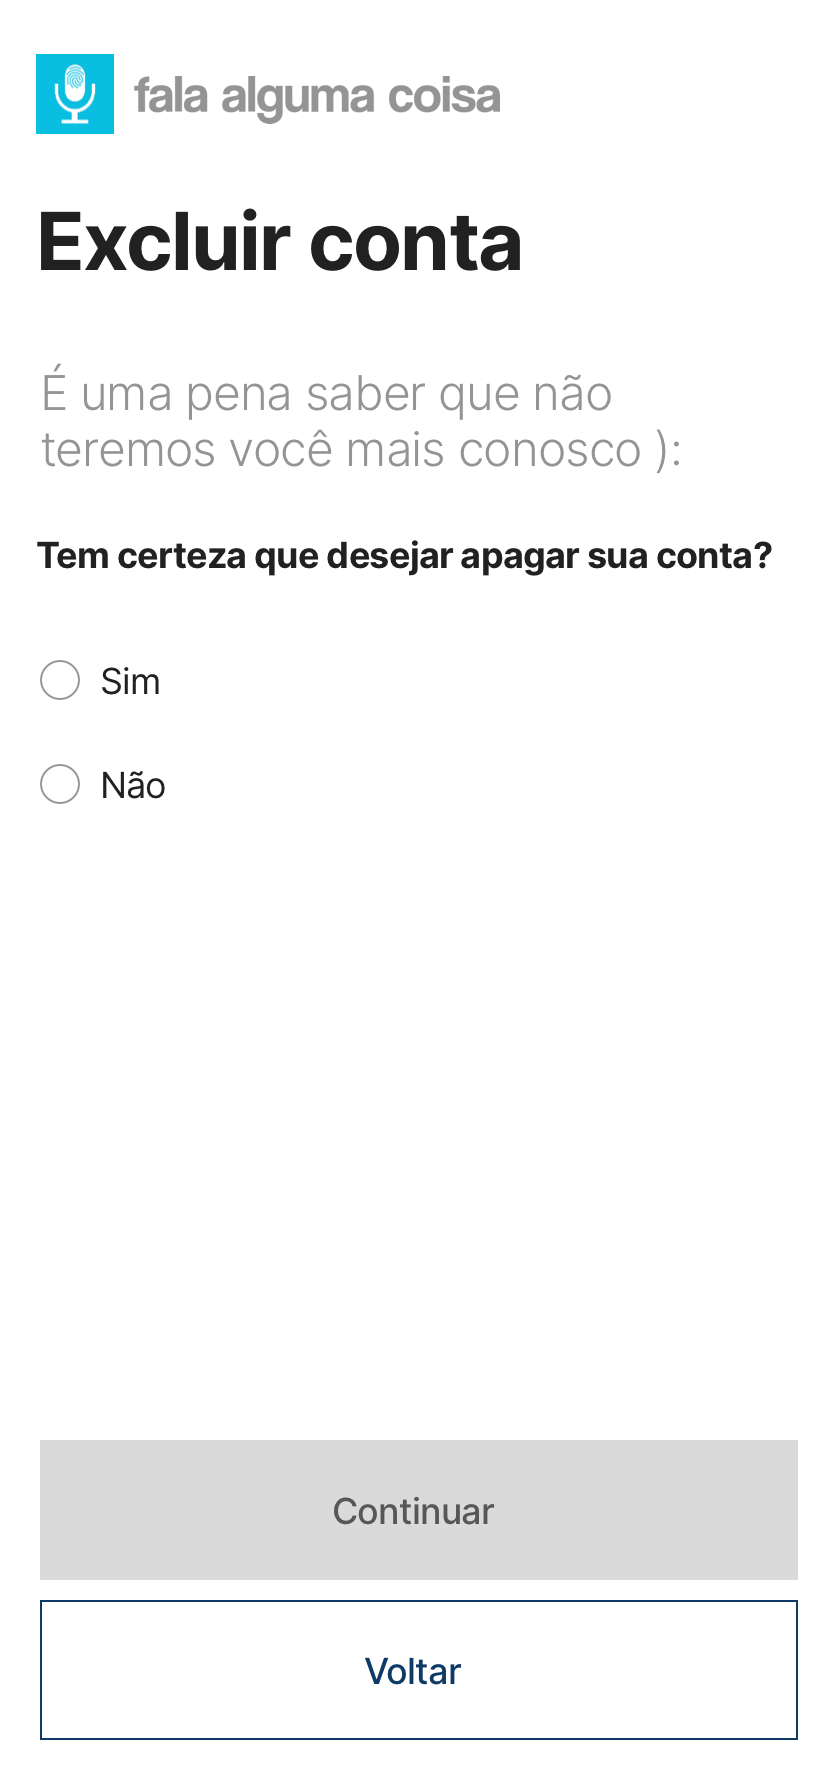
\includegraphics[width=\linewidth/2]{images/app/delete-user/FinishAccount1.0.png}}
    \caption*{Source: Author}
    \label{fig:falealgumacoisa-delete-user-data-page-design}
\end{figure}

\subsection{Development}

This section details the development process of the Fale Alguma Coisa app.

\subsubsection{Tools Selection}

To develop the application, a selection of tools was made. The table \ref{tab:tools-selection} details the selected tools and explains each choice.

\begin{table}[h]
    \centering
    \begin{tabular}{|c|c|c|}
        \hline Category & Selection & Explanation \\
        \hline Design & Zeplin & Easy sharing  \\ 
        \hline Desig &  & access \\ 
        \hline Galaxy Zoo & access & access \\ 
        \hline Christmas Audubom Birdwatch & access & access \\ \hline 
    \end{tabular}
    \caption{Contribution for online citizen science projects}
    \label{tab:cs-contributions}
\end{table}


\section{General Public Submission}
\label{sec:proposal-public-submission}

\section{Data Analysis}
\label{sec:proposal-data-analysis}

\section{Data Publication}
\label{sec:proposal-data-publication}